Students built a full voltage regulator in two preliminary stages: one to test
the bridge rectifier on its own, and one to test the voltage regulator IC.  The
design process for each of these stages is explained below.

\subsection{Bridge Rectifier}
In order to output a constant DC voltage, the AC component of
the~\SI{120}{\volt} input must first be removed.  After passing the input
through a~10:1 transformer, the input signal is routed through a configuration
of PN junctions known as a bridge rectifier.  This configuration allows current
to flow through its output resistor in only one direction, thus removing the AC
characteristics from the signal in favor of a varying DC one.  Such a circuit
is shown in Figure~\ref{fig:bridgeSchem}.
%
\begin{figure}[H]
	\centering
	\begin{circuitikz}
	\draw (0,0) node[transformer core] (T) {\qquad \SI{12}{\volt}}
	(T.A2) to [short] ++(-.5, 0)
	to [vsourcesin, l=\SI{120}{\volt} @ \SI{60}{\hertz}] ($(T.A1) - (.5,0)$)
	to [short] (T.A1)
	(T.base) node{10:1}

	% bridge rectifier (left half)
	(T.B1) to [short] ++(2.5,0) node (bridgeTop) {}
	to [Do] ++(30pt,-30pt)  % gota love non-sane measurements
	(T.B2) to [short] ++(2.5,0) node (bridgeBottom) {}
	to [Do, -*] ++(30pt, 30pt)
	% load resistor
	to [short] ++(2,0) node (loadTop) {}
	to [R, i=$i$, l=$R_\text{C}$] ++(0, -2) node[ground] (loadBottom) {}
	to [short, *-] ++($(-2, 0) + (-60pt, 0)$)
	% bridge rectifier (right half)
	to [short] ++(0, 2) node (bridgeLeft) {}
	to [Do, *-] (bridgeTop)
	(bridgeLeft) to [Do] (bridgeBottom)

	% output terminals
	(loadTop) to [short, -o] ++(1, 0)
	to [open, v^=$V_\text{L}$] ++(0, -2)
	to [short, o-] (loadBottom);

	% capacitor
	\draw[densely dashed]
		($(loadTop) - (1, 0)$) to [C, l_=$C_1$ ] ($(loadBottom) - (1, 0)$);

\end{circuitikz}

	\parbox{.6\textwidth}{
	\caption{Bridge rectifier schematic as provided in the lab three
	instructions.  Note that $C_1$ is added at a later period and is not part
	of the bridge rectifier circuit.}
	\label{fig:bridgeSchem}}
\end{figure}
%
The bridge rectifier configuration here was replaced with an IC that contains
the same parts, and the value of~$R_C$ was provided as~\SI{1}{\kilo\ohm}.  The
input and output of the bridge rectifier (after the signal passes through the
transformer) is shown in Figure~\ref{fig:bridgeRectOut} for the case that the
input signal is defined by~$12 \sin(60t)$.  Note the differences between this
waveform and the half-wave rectifier built in lab one.
%
\begin{figure}[H]
	\centering
	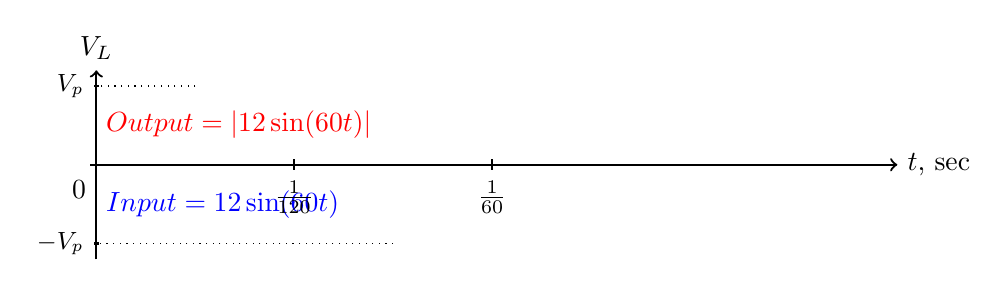
\begin{tikzpicture}[domain=0:8*pi, xscale=.4]
    %\draw[very thin,color=gray] (-0.1,-1.1) grid (8*pi, 1.1);
    \draw[->, thick] (-0.2,0) -- (8*pi+.3,0) node[right] {$t$, sec};
    \draw[->, thick] (0,-1.2) -- (0,1.2) node[above] {$V_L$};
    \draw[color=blue] plot[id=sin,samples=1000] function{sin(.5 * x)}
        node[below right, yshift=-.5\baselineskip] {$\text{Input} = 12 \sin(60 t)$};
    \draw[color=red, dashed] plot[id=abs-sin,samples=1000] function{abs(sin(.5 * x))}
        node[above right, yshift=.5\baselineskip] {$\text{Output} = \left| 12 \sin(60 t) \right|$};

	% vertical axis values
	\draw[dotted] (pi, 1) -- (0, 1);
	\draw[thick] (2pt, 1) -- (-2pt, 1) node[anchor=east] {\small$V_p$};

	\draw[dotted] (3*pi, -1) -- (0, -1);
	\draw[thick] (2pt, -1) -- (-2pt, -1) node[anchor=east] {\small$-V_p$};

	% tics
	\draw[thick] (0, 2pt) -- (0, -2pt) node[anchor=north east] {0};
	\draw[thick] (2*pi, 2pt) -- (2*pi, -2pt) node[anchor=north] {$\frac{1}{120}$};
	\draw[thick] (4*pi, 2pt) -- (4*pi, -2pt) node[anchor=north] {$\frac{1}{60}$};
\end{tikzpicture}

	\parbox{.6\textwidth}{
	\caption{Theoretical input and output for a bridge rectifier such as the
	one shown in Figure~\ref{fig:bridgeSchem}.  The input is shown in blue with
	a solid line, whereas the output is shown in red with a dashed line.}
	\label{fig:bridgeRectOut}
	}
\end{figure}
%
As is clearly shown, the period of the output signal is twice that of the
input, or in this case~$\frac{1}{120}$\si{\second} and the average value of the
output is, as intuition would dictate, also twice the average of the input,
at~$V_\text{avg} = \frac{2 V_p}{\pi}$.  Conversely, the peak value of the
output is calculated using the same method as the input,
where~$V_P=\sqrt{2}V_\mathrm{RMS}$.

\subsection{Filtered Rectifier}
The bridge rectifier shown in Figure~\ref{fig:bridgeSchem} does not by any
means resemble a constant DC voltage.  To fix this, a filtering capacitor
(drawn in dashed lines) is installed in parallel with the load resistor.  If
the value of the capacitor is chosen such that the time constant~$RC$ is much
larger than the period~$T$ of the signal it filters, then a significant
improvement in output consistency results, as displayed in
Figure~\ref{fig:bridgeRectOutFilt}.  In the experiment, the value of~$C_1$ was
provided twice: once as~\SI{1}{\micro\farad} and as~\SI{100}{\micro\farad}.
%
\begin{figure}[H]
	\centering
	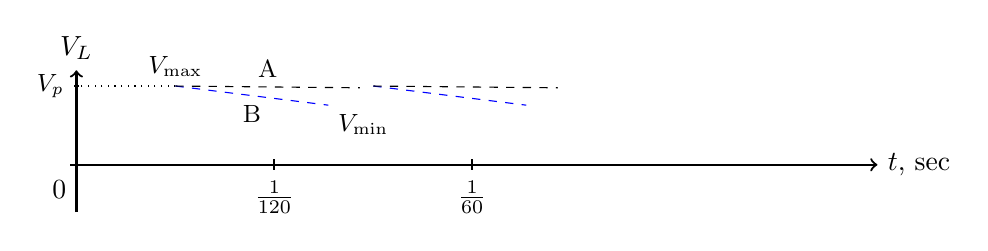
\begin{tikzpicture}[domain=0:8*pi, xscale=.4]
    \draw[->, thick] (-0.2,0) -- (8*pi+.3,0) node[right] {$t$, sec};
    \draw[->, thick] (0,-.6) -- (0,1.2) node[above] {$V_L$};
    \draw[color=red] plot[id=abs-sin,samples=1000] function{abs(sin(.5 * x))};

	% discharge lines
	\draw[color=blue, dashed] (pi,1) -- coordinate (b mid) (8, 0.75680);
	\draw[color=black, dashed] (pi,1) -- coordinate (a mid) (9, 0.97753);
	\node[above] at (a mid) {\small A};
	\node[below] at (b mid) {\small B};
	\draw[color=blue, dashed] (3*pi,1) -- (2*pi+8, 0.75680);
	\draw[color=black, dashed] (3*pi,1) -- (2*pi+9, 0.97753);
	\node[above] at (pi, 1) {\small$V_\mathrm{max}$};
	\node[anchor=north west] at (8, 0.75680) {\small$V_\mathrm{min}$};


	% vertical axis values
	\draw[dotted] (pi, 1) -- (0, 1);
	\draw[thick] (2pt, 1) -- (-2pt, 1) node[anchor=east] {\small$V_p$};

	% tics
	\draw[thick] (0, 2pt) -- (0, -2pt) node[anchor=north east] {0};
	\draw[thick] (2*pi, 2pt) -- (2*pi, -2pt) node[anchor=north] {$\frac{1}{120}$};
	\draw[thick] (4*pi, 2pt) -- (4*pi, -2pt) node[anchor=north] {$\frac{1}{60}$};
\end{tikzpicture}

	\parbox{.6\textwidth}{
	\caption{Output of the filtered bridge rectifier; waveform A depicts a
	large~RC value compared to~$T$, while waveform B depicts a small one.}
	\label{fig:bridgeRectOutFilt}
	}
\end{figure}
%
Whereas in the unfiltered case the average value of the output was~$\frac{2
V_p}{\pi}$, the DC level of the filtered signal is measured as halfway between
the maximum and minimum values shown in Figure~\ref{fig:bridgeRectOutFilt}.
Additionally, the ``ripple voltage,''~$V_r$ is greatly reduced here, as it is
calculated by~$V_\text{max} - V_\text{min}$.  This is a tremendous improvement
over the bridge rectifier alone, but will be improved further by passing this
output to an~LM723 voltage regulation IC.

\subsection{IC}
The voltage regulator integrated circuit was provided on a breakout board with
several of its external components already installed.  Students were provided
with a nominal value for~$R_2$ of~\SI{10}{\kilo\ohm}, and were told to
calculate~$R_1$ based on the measured value of~$V_\text{ref}$ and the design
goal of~$V_\text{out} = $\SI{8}{\volt}, using the equation
%
\begin{equation}
	V_\text{out} = \frac{R_1 + R_2}{R_2} V_\text{ref} \quad \text{.}
	\label{eq:calcR1}
\end{equation}
%
After adjusting a~\SI{2}{\kilo\ohm} potentiometer to the correct value, the
circuit shown in Figure~\ref{fig:icSchem} was built, utilizing the provided
breakout board for the IC, input and output connections,~$C_1$, and~$R_3$.
%
\begin{figure}[H]
	\centering
	\begin{circuitikz}
	\tikzstyle{bottomPin} = [anchor=west, rotate=90]
	\tikzstyle{topPin}    = [anchor=east, rotate=90]

	% body
	\draw[ultra thick] (-1.5,-1) rectangle (1.5,1);

	% top pins
	\draw
	( -1, 1) node[topPin] (13) {Comp}
	(-.5, 1) node[topPin] (12) {V+}
	(  0, 1) node[topPin] (11) {$\text{V}_\text{C}$}
	( .5, 1) node[topPin] (10) {$\text{V}_\text{out}$}
	(  1, 1) node[topPin] (9)  {$\text{V}_\text{Z}$}


	% bottom pins
	(-1.25, -1) node[bottomPin] (2) {$\text{I}_\text{lim}$}
	( -.75, -1) node[bottomPin] (3) {$\text{I}_\text{sense}$}
	( -.25, -1) node[bottomPin] (4) {In--}
	(  .25, -1) node[bottomPin] (5) {In+}
	(  .75, -1) node[bottomPin] (6) {$\text{V}_\text{ref}$}
	( 1.25, -1) node[bottomPin] (7) {V--};

\end{circuitikz}

	\parbox{.6\textwidth}{
	\caption{Voltage regulator integrated circuit schematic, as provided by the
	lab instructions.~$R_1$ was calculated by the student based on the
	reference voltage of his or her specific breakout board, whereas the value
	of~$R_2$ was provided as~\SI{2}{\kilo\ohm}}
	\label{fig:icSchem}
	}
\end{figure}
%
This board was initially powered by a constant DC signal of~\SI{18}{\volt} from
the lab power supply, thus ensuring that the IC functioned correctly with the
chosen values.  This also allowed the value of~$R_1$ to be tuned further,
providing an output of~\SI{8}{\volt}.  Once this procedure had been completed,
a resistor was placed in parallel with both~$R_1$ and~$R_2$ to provide an
adequate load and the line regulation (change in output per change in input)
was calculated.  Finally, the load regulation (change in output per change in
load) was calculated by replacing the varying source for a static one, and the
static load resistor for a decade box.

The results of both the load and line regulation tests can be seen in
Figures~\ref{fig:vrLineReg} and~\ref{fig:vrLoadReg}.

\subsection{Full Regulator}
At this point in the experiment, the completed voltage regulator was ready to
be constructed by simply wiring the output of the filtered bridge rectifier to
the input of the IC breakout board.  This circuit is shown in
Figure~\ref{fig:fullSchem} for clarity.
%
\begin{figure}[H]
	\centering
	\scalebox{.75}{ % comment this line if you want to put this on its own page in
                % a sideways environment
\begin{circuitikz}
	\draw (0,0) node[transformer core] (T) {\qquad \SI{12}{\volt}}
	(T.A2) to [short] ++(-.5, 0)
	to [vsourcesin, l=\SI{120}{\volt} @ \SI{60}{\hertz}] ($(T.A1) - (.5,0)$)
	to [short] (T.A1)
	(T.base) node{10:1}

	% bridge rectifier (left half)
	(T.B1) to [short] ++(2.5,0) node (bridgeTop) {}
	to [Do] ++(30pt,-30pt)  % gota love non-sane measurements
	(T.B2) to [short] ++(2.5,0) node (bridgeBottom) {}
	to [Do, -*] ++(30pt, 30pt)
	% load resistor
	to [short] ++(2,0) node (loadTop) {}
	to [R, i=$i$, l=$R_\text{C}$] ++(0, -2) node[ground] (loadBottom) {}
	to [short, *-] ++($(-2, 0) + (-60pt, 0)$)
	% bridge rectifier (right half)
	to [short] ++(0, 2) node (bridgeLeft) {}
	to [Do, *-] (bridgeTop)
	(bridgeLeft) to [Do] (bridgeBottom)

	% output terminals
	(loadTop) to [short, -o] ++(1, 0) node (rect-out+) {}
	to [open] ++(0, -2) node (rect-out-) {}
	to [short, o-] (loadBottom);

	% capacitor
	\draw[densely dashed]
		($(loadTop) - (1, 0)$) to [C, l_=$C_1$ ] ($(loadBottom) - (1, 0)$);





	\begin{scope}[shift={(12, -1.5)}]

	\tikzstyle{bottomPin} = [anchor=west, rotate=90]
	\tikzstyle{topPin}    = [anchor=east, rotate=90]

	% body
	\draw[ultra thick] (-1.5,-1) rectangle (1.5,1);

	% IC label
	\draw (1.5, 1) node[anchor=north west] {LM723};

	% top pins
	\draw
	( -1, 1) node[topPin] {Comp}
	(-.5, 1) node[topPin] {V+}
	(  0, 1) node[topPin] {$\text{V}_\text{C}$}
	( .5, 1) node[topPin] {$\text{V}_\text{out}$}
	(  1, 1) node[topPin] {$\text{V}_\text{Z}$}


	% bottom pins
	(-1.25, -1) node[bottomPin] {$\text{I}_\text{lim}$}
	( -.75, -1) node[bottomPin] {$\text{I}_\text{sense}$}
	( -.25, -1) node[bottomPin] {In--}
	(  .25, -1) node[bottomPin] {In+}
	(  .75, -1) node[bottomPin] {$\text{V}_\text{ref}$}
	( 1.25, -1) node[bottomPin] {V--};

	% lines
	\draw
	% C1
	(-1,1) to [short] ++(0, .5)
	to [short] ++(-1.5, 0)
	to [C, l_=$C_1$] ++(0, -3.5)
	to [short, -*] ++(2.25, 0)

	% Vin +
	(-.5, 1) to [short] ++(0, 1)
	to [short, -o] ++(-3, 0) node (ic-in+) {} node[anchor=south] {$\text{V}_\text{in}$+}

	% VC
	(0, 1) to [short] ++(0, .5)
	to [short, -*] ++(-.5, 0)

	% Vout
	(.5, 1) to [short] ++(0, .5)
	to [short, -*] ++(3, 0) node (vout-junc) {}
	to [short, -o] ++(0, 1) node[anchor=south] {$\text{V}_\text{out}$}

	% In -
	(-.25, -1) to [short] ++(0, -2)
	to [short] ++(2.25, 0)
	to [short] ++(0, 3)
	to [short, -*] ++(1.5, 0)

	% R3
	(.25, -1) to [short] ++(0, -.5)
	to [short] ++(-.25, 0)
	to [short] ++(0, -.75)
	to [R, l_=$R_3$] ++(1.5, 0)
	to [short] ++(0, .5)
	to [short] ++(-.75, 0)
	to [short] (.75, -1)

	% V-
	(1.25, -1) to [short] ++(0, -.5)
	to [short, -*] ++(2.25, 0)

	% vout -> ... -> Vin -
	(vout-junc) to [R, l^=$R_1$] ++(0, -1.5)
	to [R, l^=$R_2$] ++(0, -1.5)
	to [short] ++(0, -2) node (gnd-right) {}
	to [short] ++(-3.5, 0) node (gnd-left) {}
	to [short, -o] ++(-3.5, 0) node (ic-in-) {} node[anchor=north] {$\text{V}_\text{in}$--}

	% grounds
	(gnd-right) to [short] ++(0, -.25) node[ground] {}
	(gnd-left)  to [short] ++(0, -.25) node[ground] {};

	% non-connected
	\draw[-|] (-1.25, -1) -- ++(0, -.25);
	\draw[-|] (-.75,  -1) -- ++(0, -.25);
	\draw[-|] (   1,   1) -- ++(0,  .25);


	\end{scope}

	% interconnect  -- this is a major hack...
	\draw (rect-out+) |- (ic-in+)
	(rect-out+) to [short, o-] ++(0, .5)
	(ic-in+) to [short, o-] ++(-.5, 0)
	(rect-out-) |- (ic-in-)
	(rect-out-) to [short, o-] ++(0, -.5)
	(ic-in-) to [short, o-] ++(-.5, 0);

\end{circuitikz}
}

	\caption{}
	\label{fig:fullSchem}
\end{figure}
%
The load regulation for this circuit was measured, using a decade box across
resistors one and two to modulate the load.  Results of this resistance sweep
are plotted in Figure~\ref{fig:fullLoadReg}.
